\section{Classical SVM}
\label{sec:classical_svm}
\remLE{Khanh Duy write this part. Write details: ideas, models,  important concepts. Please focus on the mathematical logic and flow of writting.}


In this section, we revisit the ideas as well as the important concepts in the models of Support Vector Machines that serve as the theoretical foundation for our tree-based variant studied in the next section.


\subsection{Concepts and models SVM}
Let us consider a classification dataset $\{(x_i,y_i)\}^n_{i=1}$ where $x_i \in \mathbb{R}^d$ represents the feature vectors and $y_i\in \{-1,+1\}$ denotes the class labels. The key idea of SVM is to find a separating hyperplane that divides the feature space into two disjoint regions corresponding to the two classes.

In $\mathbb{R}^d$, a hyperplane can be expressed as:
\[(H):w^Tx+b=0,\] where $w\in \mathbb{R}^d$ is the normal vector of the hyperplane, $b$ là bias.
\subsection{Determining the separating hyperplane}
To define the separating hyperplane in a binary classification problem, we seek $(w,b)$ such that
\[(H):w^Tx+b=0,\] where $w\in \mathbb{R}^d$ is the normal vector and $b$ is bias.

Because the separating hyperplane cannot pass through any training point, we introduce two parallel supporting hyperplanes:
\[(H_+): \ w^Tx+b=\delta, \hspace{2cm} (H_-): \ w^Tx+b=-\delta,\] with $\delta >0$, where $H_+$ passes through the closest point(s) belonging to class $+1$ and $H_-$ passes through the closest point(s) belonging to class $-1$.

Since $\delta > 0$ is an arbitrary positive constant, if $(w,b,\delta)$ satisfies the separation constraints, then $(\lambda w,\lambda,\lambda\delta)$ also satisfies them for any $\lambda > 0$. Therefore, we can normalize $\delta = 1$ without losing generality. Under this normalization, the two supporting hyperplanes can be rewritten as:
\[
(H_+): \ w^\top x + b = 1, \qquad 
(H_-): \ w^\top x + b = -1.
\]
Thus, any data point $x_i$ that satisfies $w^Tx+b\ge 1$ is classified as belonging to the positive class $(y_i=+1)$, whereas any point satisfying $w^Tx+b\le -1$ is classified as belonging to the negative class $(y_i=-1)$. Combining both cases, the classification constraints can be expressed compactly as
\[y_i(w^Tx+b)\ge 1.\]

\subsection{Max margin Method}
At this point, the data points $x_i$ are located on two opposite sides of the separating hyperplane.
However, since there exist infinitely many hyperplanes that can separate the two classes, the next problem is to select the optimal hyperplane that also minimizes the risk of overfitting.

\begin{figure}[H]
    \centering
        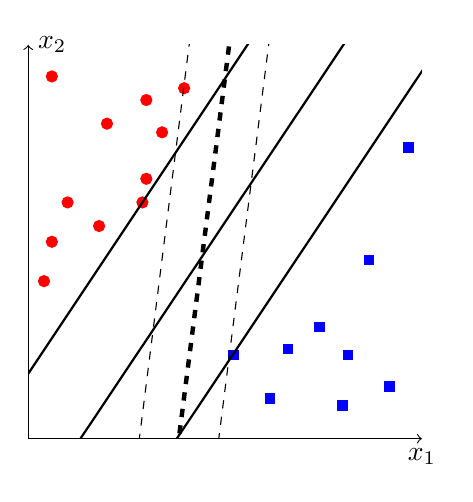
\begin{tikzpicture}[scale=1]
        %Trục
            \draw [->] (0,0)--(5,0) node [below]{$x_1$};
            \draw [->] (0,0)--(0,5) node [right]{$x_2$};
        %Điểm dữ liệu +1
        \foreach \x/\y in{
        1/4, 0.5/3, 0.3/4.6, 1.5/4.3, 1.7/3.89, 1.5/3.3, 1.45/3, 0.2/2, 0.3/2.5, 0.9/2.7,1.98/4.45
        }{\filldraw[red] (\x,\y) circle (2pt);}
        %Điểm dữ liệu -1
        \foreach \u/\v in{
        4/1, 2.55/1, 4.27/2.21, 3.64/1.36, 4.53/0.6, 3.93/.36, 4.77/3.64,3.01/.45, 3.24/1.08
        }{\filldraw[blue] (\u,\v) rectangle ++(0.12,0.12);}
            
        %Siêu phẳng
        \begin{scope}
        \clip (0,0) rectangle (5,5);
        \draw[thick] (-0.39,0.24)--(3.45,6);
        \draw[thick] (0.45,-0.32)--(4.67,6);
        \draw[thick] (1.3,-0.88)--(5.89,6);

        \draw[dashed] (1.3,-0.88)--(2.17,6);
        \draw[ultra thick, dashed] (1.76,-1.19)--(2.68,6);
        \draw[dashed] (2.23,-1.5)--(3.18,6);
        \end{scope}
        \end{tikzpicture}
    
    \caption{Maximum-margin classification in $\mathbb{R}^2$}
\end{figure}

When the two classes are close to each other, the model is more prone to overfitting because small variations in the data can lead to significant changes in the separating hyperplane. To improve generalization, our aim is to maximize the distance between the two classes, referred to as the margin. This principle is known as the maximum-margin method.

We define the width of the margin as $\Delta$. By definition, $\Delta$ is the sum of the distances from the separating hyperplane $(H)$ to the two supporting hyperplanes $(H_+)$ and $(H_-)$. Formally:
\[\Delta=d(H,x_+)+d(H,x_-),\] where $x_+ \in (H_+)$ and $x_-\in (H_-).$

For any point $x_+ \in (H_+)$, we have the following:
\[d(H,x_+)=\dfrac{|w^Tx_++b|}{\|w\|_2}=\dfrac{1}{\|w\|_2},\]
and similarly, for any $x_-\in (H_-):$ 
\[d(H,x_-)=\dfrac{|w^Tx_-+b|}{\|w\|_2}=\dfrac{1}{\|w\|_2}.\]
Therefore, the margin is given by:
\[\Delta = \dfrac{1}{\|w\|_2}+\dfrac{1}{\|w\|_2}=\dfrac{2}{\|w\|_2}.\]

Since we aim to construct a classifier based on the maximum-margin principle, the optimization objective is to maximize the margin $\Delta$:
\[\max_{w,b}\Delta=\max_{w,b}\dfrac{2}{\|w\|_2}\]
Maximizing the margin is equivalent to minimizing $\|w\|_2$, leading to the equivalent problem:
\[\min_{w,b} \dfrac{1}{2}\|w\|_2\]
 However, the objective function $\|w\|_2$ is non-differentiable, which can cause computational difficulties. To overcome this, we square the norm, yielding a smooth and differentiable objective function. Thus, the optimization problem is model as follows:
 \begin{align}
\min_{w,b} \quad &\frac{1}{2}\|w\|^2_2 \\
\text{s.t.} \quad &y_i(w^T x_i + b) \geq 1, \quad i = 1,\ldots,n
\end{align}
\subsection{Hard margin and soft margin SVM}
In practice, even when there is a separate hyperplane, a few data points can significantly deteriorate the classification performance.
However, if we allow for the ignoring of some of these points, we can obtain a better separating hyperplane with improved generalization capability.
Such points are referred to as noisy points (see Figure \ref{Noisy point}).

\begin{figure}[H]
    \centering
        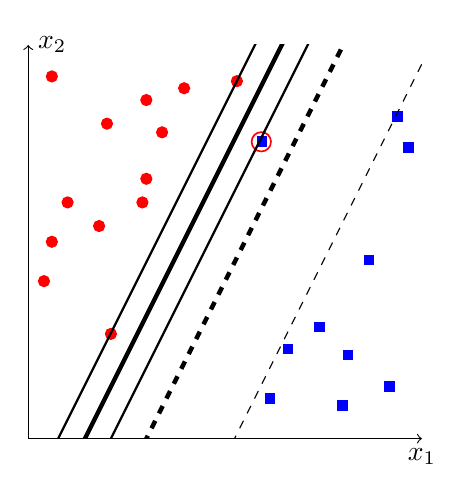
\begin{tikzpicture}[scale=1]
        %Trục
            \draw [->] (0,0)--(5,0) node [below]{$x_1$};
            \draw [->] (0,0)--(0,5) node [right]{$x_2$};
        %Điểm dữ liệu +1
        \foreach \x/\y in{
        1/4, 0.5/3, 0.3/4.6, 1.5/4.3, 1.7/3.89, 1.5/3.3, 1.45/3, 0.2/2, 0.3/2.5, 0.9/2.7,1.98/4.45, 2.65/4.54, 1.05/1.33
        }{\filldraw[red] (\x,\y) circle (2pt);}
        %Điểm dữ liệu -1
        \foreach \u/\v in{
        4/1, 4.27/2.21, 3.64/1.36, 4.53/0.6, 3.93/.36, 4.77/3.64,3.01/.45, 3.24/1.08, 2.91/3.71, 4.63/4.03
        }{\filldraw[blue] (\u,\v) rectangle ++(0.12,0.12);}
            \draw[red,semithick] (2.96,3.77) circle (3.5pt);
        %Siêu phẳng
        \begin{scope}
        \clip (0,0) rectangle (5,5);
        \draw[thick] (-.12,-1)--(3.38,6);
        \draw[dashed,ultra thick] (1,-1)--(4.5,6);
        \draw[dashed] (2.12,-1)--(5.62,6) ;

        \draw[ultra thick] (0.22,-1)--(3.72,6);
        \draw[thick] (.55,-1)--(4.05,6);
        \end{scope}
        \end{tikzpicture}
    \caption{Optimal hyperplane with noisy point in $\mathbb{R}^2$}
    \label{Noisy point}
\end{figure}

If we do not ignore noisy points and enforce perfect classification for all samples, the problem model is called a hard-margin SVM, corresponding to the original strict separability constraints:
\[y_i(w^Tx_i+b)\ge 1, ~ \forall i=1,2,3,...,n.\]

Conversely, if we allow misclassification of a small number of noisy points to achieve a better overall separation, we adopt the soft-margin SVM model.

In the soft-margin SVM model, we allow some data points to violate the margin constraints in order to achieve better generalization and robustness to noise. Each data point $(x_i,y_i)$ falls into one of the following three case:
\begin{enumerate}[label=Case~\arabic*.]
    \item Correctly classified and outside the margin
    \[y_i(w^Tx_i+b)\ge 1\]
    These points lie outside the margin boundaries and are classified correctly.
    \item Correctly classified but inside the margin
     \[0\le y_i(w^Tx_i+b)\le 1\]
     These points are still classified correctly but lie inside the margin, thus slightly violating the margin constraint.
    \item Misclassified points
     \[y_i(w^Tx_i+b) < 0 \]
     These points lie on the wrong side of the separating hyperplane, meaning they are classified incorrectly.
\end{enumerate}

\begin{figure}[H]
    \centering
        \begin{tikzpicture}[scale=1.3]
        %Trục
            \draw [->] (0,0)--(4,0) node [below]{$x_1$};
            \draw [->] (0,0)--(0,4) node [right]{$x_2$};
        %Điểm dữ liệu +1
        \foreach \x/\y in{
        0.5/3, 1.7/3.7, 1.5/3.3, 1.45/3, 0.2/2, 0.3/2.5, 0.9/2.7, 2/1
        }{\filldraw[red] (\x,\y) circle (2pt);}
        %Điểm dữ liệu -1
        \foreach \u/\v in{
        2.55/1, 3.64/1.36, 3.5/.36, 3.01/.45, 3.24/1.08, 0.9/3, 3/3
        }{\filldraw[blue] (\u,\v) rectangle ++(0.12,0.12);}
        
        \coordinate (H) at ($(-.39,.24)!(2,1)!(3.45,6)$);
        \draw[dashed,thick] (H)--(2,1);

        \coordinate (K) at ($(1.3,-.88)!(0.9,3)!(5.89,6)$);
        \draw[dashed,thick] (K)--(1.01,3);

        \coordinate (I) at ($(1.3,-.88)!(3,3)!(5.89,6)$);
        \draw[dashed, thick] (I)--(3.11,3);
        %Siêu phẳng
        \begin{scope}
        \clip (0,0) rectangle (4,4);
        \draw[thick] (-0.39,0.24)--(3.45,6);
        \draw[ultra thick] (0.45,-0.32)--(4.67,6);
        \draw[thick] (1.3,-0.88)--(5.89,6);
        \end{scope}
        \end{tikzpicture}
    \caption{Cases with slack variable}
\end{figure}
To unify the three cases discussed above, we introduce a slack variable $\xi\ge0$
\[y_i(w^Tx_i+b)\ge 1-\xi_i,\ \forall i=1,2,...,n.\]
where:\\
Case 1 is $\xi_i=0$\\
Case 2 is $0<\xi_i\le 1$\\
Case 3 is $\xi_i>1$

With the introduction of the slack variables $\xi_i\ge 0$, the optimization problem of the soft-margin SVM becomes finding the optimal $(w,b,\xi)$ that minimizes the following objective function:
\begin{align}
\min_{w,b,\xi} \quad &\frac{1}{2}\|w\|^2 + C\sum_{i=1}^n \xi_i \\
\text{s.t.} \quad &y_i(w^T x_i + b) \geq 1 - \xi_i, \quad i = 1,\ldots,n \\
&\xi_i \geq 0, \quad i = 1,\ldots,n
\end{align}
where $C > 0$ is the regularization parameter that balances between margin maximization and training error minimization.

Notice that the slack variable $\xi$ measures the degree of violation of the restriction. By rearranging, we obtain:
\[\xi_i\ge 1-y_i(w^Tx_i+b), ~ \xi_i\ge 0\]
Thus, at the optimum,
\[\xi_i=\max(1-y_i(w^Tx_i+b),0)\]
Substituting this back into the objective function yields the unconstrained optimization problem:
\[\min_{w,b}\dfrac{1}{2}\|w\|^2_2+C\sum_{i=1}^n\max(1-y_i(w^Tx_i+b),0)\]
The second term,
\[\mathcal{L}=\max(1-y_if(x_i),0),\]
is called hinge loss, where $f(x)=w^Tx+b$ 




% \subsection{Hard margin SVM}


% Given a labeled training dataset $\{(x_i, y_i)\}_{i=1}^n$ where $x_i \in \mathbb{R}^d$ are feature vectors and $y_i \in \{-1, +1\}$ are binary class labels, the goal of SVM is to find a hyperplane, say $w^T x + b =0$ for $w \in \RR^d$ and $b \in \RR$, that optimally separates the two classes, in the sense that 

% \begin{align*}
%     w^T x + b & \geq 1, \quad \forall y_i =+1\\
%     w^T x + b & \leq -1, \quad \forall y_i =-1
% \end{align*}

% The margin is defined as the distance between the two hyperplanes $w^T x + b=1$ and $w^T x + b=-1$, which is $\frac{2}{\|w\|_2}$. SVM model seeks the separating hyperplane with maximal margin.
% This leads to the following optimization problem:

% \begin{align}
% \min_{w,b} \quad &\frac{1}{2}\|w\|^2 \\
% \text{s.t.} \quad &y_i(w^T x_i + b) \geq 1, \quad i = 1,\ldots,n
% \end{align}

% The constraints ensure that all training points are correctly classified with at least unit distance from the decision boundary.

% The point (or equivalently considered as a vector) $s\in V_+$ and $p\in V_+$ are said to be positive and negative support vector, respectively, if they are on the supporting hyperplane, \ie
% \begin{align*}
%     w^s + b &= 1\\
%     w^p + b &= -1.\\
% \end{align*}
% Hence the name SVM.


% \subsection{Soft Margin SVM}

% To handle non-separable cases, the soft margin SVM introduces slack variables $\xi_i \geq 0$:

% \begin{align}
% \min_{w,b,\xi} \quad &\frac{1}{2}\|w\|^2 + C\sum_{i=1}^n \xi_i \\
% \text{s.t.} \quad &y_i(w^T x_i + b) \geq 1 - \xi_i, \quad i = 1,\ldots,n \\
% &\xi_i \geq 0, \quad i = 1,\ldots,n
% \end{align}

% where $C > 0$ is the regularization parameter that balances between margin maximization and training error minimization.



% \begin{remark}[Kernel method]
%     To handle nonlinear classification, SVM can be extended using kernel functions $K(x_i, x_j) = \phi(x_i)^T \phi(x_j)$ that implicitly map data to higher-dimensional feature spaces. Common kernels include:

%     \begin{itemize}
%     \item \textbf{Linear kernel}: $K(x_i, x_j) = x_i^T x_j$
%     \item \textbf{RBF kernel}: $K(x_i, x_j) = \exp(-\gamma \|x_i - x_j\|^2)$
%     \item \textbf{Polynomial kernel}: $K(x_i, x_j) = (x_i^T x_j + c)^p$
%     \end{itemize}
% \end{remark}






\subsection{New interpretation of SVM based on support vectors}
\remLE{Le do this part}
In this section, we rewrite the soft-margin SVM model in term of support vectors. This will lay the foundation for our SVM model on tree in the next section. 

Define 
\begin{equation*}
    \sigma(x_i) = w^T x_i + b
\end{equation*}
and 
\begin{equation*}
    d(x_i, x_j) = \sigma(x_i) - \sigma(x_j)
\end{equation*}

Let $s \in V_+$ and $p \in V_-$ be two support vectors, then the margin is given by the distance between $s$ and $p$, 
\begin{equation*}
    \frac{2}{\|w\|_2}
    = \frac{(w^T s + b) - (w^T p + b)}{\|w\|_2}
    = \frac{d(s, p)}{\|w\|_2}.
\end{equation*} 

In the soft margin SVM, the noise can also be written in terms of $s$ and $p$ as follows. For $x_i \in V_+$, we should have 
\begin{align*}
    \xi_i & = 1 - (w^T x_i + b), \forall x_i \in V_+\\
    & = \sigma(s)  - \sigma(x_i)\\
    & = d(s, x_i)\\
\end{align*}




